\input{common/preamble.tex}

\begin{document}

\includepdf[pages={1}]{src/title.pdf}

\renewcommand*\contentsname{СОДЕРЖАНИЕ}
{
\setcounter{tocdepth}{3}
\tableofcontents
}
\pagebreak

\section*{ВВЕДЕНИЕ}\label{sec:introduction}
\addcontentsline{toc}{section}{Введение}

Разработка современных программных систем неразрывно связана с непрерывным ростом их сложности и уровня ответственности. В таких условиях фундаментальным этапом жизненного цикла разработки становится инженерия требований. Требования к системе представляют собой документированное описание функций, поведенческих сценариев, свойств и ограничений, которым должна удовлетворять разрабатываемая система для решения поставленных задач. Потребность в их строгом выделении обусловлена необходимостью исключить двусмысленность на этапе проектирования и, что более важно, создать объективный эталон для последующего тестирования и верификации. Без четко сформулированных требований невозможно доказать корректность работы системы, а обнаружение концептуальных ошибок на этапе эксплуатации влечет за собой критический рост издержек.

Существующие подходы к описанию требований для сложных программных систем варьируются от неформальных текстовых до строго математических. Так, легковесные методы, такие как \textit{EARS} (Easy Approach to Requirements Syntax)~\cite{ears}, предоставляют инженерам жесткие структурные шаблоны для естественного языка, но остаются слабо формализованными инструментами. С другой стороны, существуют тяжеловесные формальные методы, такие как \textit{TLA+} и \textit{B-Method}~\cite{meteor} (последний доказал свою эффективность при верификации программного обеспечения 14-й линии Парижского метрополитена). Концептуально близкими к формализму \textit{EDTL} являются подходы \textit{PSP}~\cite{psp} и \textit{PSL}~\cite{psl}: они занимают промежуточное положение, совмещая простоту использования текстовых шаблонов со строгой семантикой, пригодной для автоматической проверки моделей.

В данной работе речь будет идти об \textit{Event-Driven Temporal Logic (EDTL)}. Данный формализм спецификаций позволяет описывать поведение ПО в терминах событий (включая таймауты) и логических операций над входами и выходами, абстрагируясь от внутренней реализации и рассматривая целевую систему как «черный ящик».

Поскольку EDTL-спецификации транслируются в формулы линейной темпоральной логики (\textit{LTL}), открывается возможность для их формального анализа. Однако в процессе формирования спецификаций в результирующем наборе \textit{LTL}-формул могут возникать скрытые дефекты.

Наиболее критичным из них является противоречивость — наличие взаимно исключающих спецификаций, совместное выполнение которых невозможно (то есть конъюнкция соответствующих LTL-формул не имеет модели). Наличие даже одного конфликтующего подмножества требований делает невозможной разработку корректно функционирующей системы.

Менее очевидной, но существенной проблемой является избыточность, которая возникает, когда отдельное требование не накладывает на систему новых ограничений, поскольку является логическим следствием множества других спецификаций. Хотя избыточные требования напрямую не препятствуют реализации системы, они необоснованно усложняют модель или повышают риск внесения ошибок при её дальнейшей модификации.

В связи с этим возникает  задача автоматизированного контроля качества полученного набора требований, а именно — проверка спецификаций на непротиворечивость и отсутствие избыточности.

Для решения подобных задач традиционно применяются алгоритмы анализа подмножеств ограничений MUS (Minimal Unsatisfiable Subset), MSS (Maximal Satisfiable Subset). Среди таких алгоритмов выделяют MARCO (Mapping Regions of Constraints)~\cite{marco}, отличительными чертами которого являются выдача результирующих подмножеств(и MUS, и MSS) "на лету", а также независимость от синтаксиса проверяемых ограничений, что обеспечивает универсальность алгоритма.

% Завершение введения отдельным параграфом со сноской\footnote{Любая
%   дополнительная информация может вынесена в сноску, включая
%   форматирование \emph{текста} и формул (\(\sum_{i}^{n}{i}\)).}.

\clearpage
\pagebreak

\section{Предметная область}\label{sec:overview}
\subsection{LTL}\label{sec:ltl}

Процесс верификации моделей требует перевода неформальных требований к программной системе в строгую математическую спецификацию. Для формального описания реактивных систем, чье поведение представляет собой распределенные во времени последовательности событий, применяются темпоральные логики. В частности, линейная темпоральная логика (LTL) позволяет формулировать утверждения о свойствах путей вычислений, в отличие от логики ветвящегося времени (CTL), которая описывает свойства деревьев вычислений.

Формулы LTL интерпретируются на математических структурах, называемых моделями Крипке. Модель Крипке формально задается кортежем $M = (S, S_0, R, L)$, где $S$~--- конечное множество возможных состояний системы, $S_0 \subseteq S$~--- множество начальных состояний, $R \subseteq S \times S$~--- тотальное отношение переходов между состояниями, а $L \colon S \to 2^{AP}$~--- функция разметки, сопоставляющая каждому состоянию набор истинных в нем атомарных высказываний. Путь в модели $M$ из заданного состояния определяется как бесконечная последовательность состояний $\pi = s_0, s_1, s_2, \dots$, такая что $s_0 = s$, и для всех $i \ge 0$ выполняется условие $R(s_i, s_{i+1})$.
\vspace{\baselineskip}
\begin{definition}[Синтаксис LTL]\label{def:ltl_syntax}
    Если $\varphi$ и $\psi$~--- корректные LTL-формулы, то допустимыми являются следующие конструкции:
    \begin{itemize}
        \item атомарное высказывание $p$;
        \item логические операции: $\neg\varphi$, $\varphi \land \psi$, $\varphi \lor \psi$;
        \item темпоральные операторы:
        \begin{itemize}
            \item $X\varphi$ (NeXt)~--- свойство $\varphi$ выполняется в следующий момент времени;
            \item $F\varphi$ (Future)~--- свойство $\varphi$ когда-нибудь обязательно выполнится;
            \item $G\varphi$ (Globally)~--- свойство $\varphi$ выполняется всегда;
            \item $\varphi U \psi$ (Until)~--- свойство $\varphi$ выполняется до тех пор, пока не выполнится $\psi$.
        \end{itemize}
    \end{itemize}
\end{definition}

\begin{definition}[Семантика LTL]\label{def:ltl_semantics}
    Истинность LTL-формулы определяется на конкретном пути вычисления $\pi$. Пусть $\pi^k = s_k, s_{k+1}, \dots$~--- суффикс пути $\pi$, начинающийся с $k$-го шага. Отношение выполнимости $M, \pi \models \varphi$ (означающее, что формула $\varphi$ истинна на пути $\pi$ в модели $M$) задается индуктивно по структуре формулы:
    \begin{enumerate}
        \item $M, \pi \models p \Leftrightarrow p \in L(s)$;
        \item $M, \pi \models \neg\varphi \Leftrightarrow M, \pi \not\models \varphi$;
        \item $M, \pi \models \varphi_1 \land \varphi_2 \Leftrightarrow M, \pi \models \varphi_1$ и $M, \pi \models \varphi_2$;
        \item $M, \pi \models \varphi_1 \lor \varphi_2 \Leftrightarrow M, \pi \models \varphi_1$ или $M, \pi \models \varphi_2$;
        \item $M, \pi \models X\varphi \Leftrightarrow M, \pi^1 \models \varphi$;
        \item $M, \pi \models \varphi_1 U \varphi_2 \Leftrightarrow$ существует $k \ge 0$ такое, что $M, \pi^k \models \varphi_2$, и для всех $0 \le j < k$ верно $M, \pi^j \models \varphi_1$.
        \item $M, \pi \models F\varphi \Leftrightarrow$ существует $k \ge 0$ такое, что $M, \pi^k \models \varphi$;
        \item $M, \pi \models G\varphi \Leftrightarrow$ для всех $k \ge 0$ верно, что $M, \pi^k \models \varphi$;
    \end{enumerate}
\end{definition}

\begin{figure}[htbp]
    \centering % Эта команда центрирует всё, что находится ниже неё


\tikzset{every picture/.style={line width=0.75pt}} %set default line width to 0.75pt        

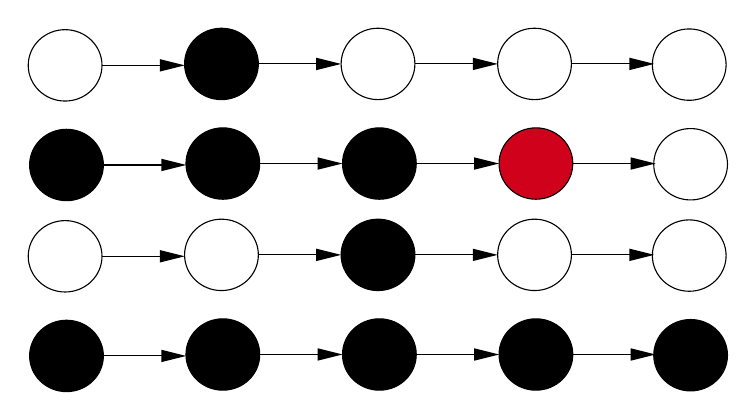
\begin{tikzpicture}[x=0.75pt,y=0.75pt,yscale=-1,xscale=1]
%uncomment if require: \path (0,242); %set diagram left start at 0, and has height of 242

%Shape: Ellipse [id:dp6353801488874232] 
\draw   (22.57,65.38) .. controls (22.57,55.89) and (30.53,48.19) .. (40.34,48.19) .. controls (50.15,48.19) and (58.11,55.89) .. (58.11,65.38) .. controls (58.11,74.88) and (50.15,82.58) .. (40.34,82.58) .. controls (30.53,82.58) and (22.57,74.88) .. (22.57,65.38) -- cycle ;
%Straight Lines [id:da6599924595958612] 
\draw    (58.11,65.38) -- (95.99,65.38) ;
\draw [shift={(97.99,65.38)}, rotate = 180] [fill={rgb, 255:red, 0; green, 0; blue, 0 }  ][line width=0.08]  [draw opacity=0] (12,-3) -- (0,0) -- (12,3) -- cycle    ;
%Shape: Ellipse [id:dp6072020367173158] 
\draw  [fill={rgb, 255:red, 0; green, 0; blue, 0 }  ,fill opacity=1 ] (97.9,64.69) .. controls (97.9,55.2) and (105.86,47.5) .. (115.67,47.5) .. controls (125.48,47.5) and (133.44,55.2) .. (133.44,64.69) .. controls (133.44,74.19) and (125.48,81.89) .. (115.67,81.89) .. controls (105.86,81.89) and (97.9,74.19) .. (97.9,64.69) -- cycle ;
%Straight Lines [id:da9951777591535165] 
\draw    (133.44,64.69) -- (171.32,64.69) ;
\draw [shift={(173.32,64.69)}, rotate = 180] [fill={rgb, 255:red, 0; green, 0; blue, 0 }  ][line width=0.08]  [draw opacity=0] (12,-3) -- (0,0) -- (12,3) -- cycle    ;
%Shape: Ellipse [id:dp008501598916548336] 
\draw   (173.32,64.69) .. controls (173.32,55.2) and (181.28,47.5) .. (191.09,47.5) .. controls (200.9,47.5) and (208.86,55.2) .. (208.86,64.69) .. controls (208.86,74.19) and (200.9,81.89) .. (191.09,81.89) .. controls (181.28,81.89) and (173.32,74.19) .. (173.32,64.69) -- cycle ;
%Straight Lines [id:da2511202980522963] 
\draw    (208.86,64.69) -- (246.74,64.69) ;
\draw [shift={(248.74,64.69)}, rotate = 180] [fill={rgb, 255:red, 0; green, 0; blue, 0 }  ][line width=0.08]  [draw opacity=0] (12,-3) -- (0,0) -- (12,3) -- cycle    ;
%Shape: Ellipse [id:dp6511748739172353] 
\draw   (248.74,64.69) .. controls (248.74,55.2) and (256.7,47.5) .. (266.51,47.5) .. controls (276.32,47.5) and (284.27,55.2) .. (284.27,64.69) .. controls (284.27,74.19) and (276.32,81.89) .. (266.51,81.89) .. controls (256.7,81.89) and (248.74,74.19) .. (248.74,64.69) -- cycle ;
%Straight Lines [id:da16390305234987546] 
\draw    (284.27,64.69) -- (322.16,64.69) ;
\draw [shift={(324.16,64.69)}, rotate = 180] [fill={rgb, 255:red, 0; green, 0; blue, 0 }  ][line width=0.08]  [draw opacity=0] (12,-3) -- (0,0) -- (12,3) -- cycle    ;
%Shape: Ellipse [id:dp4145305973075424] 
\draw   (323.27,65.04) .. controls (323.27,55.54) and (331.23,47.84) .. (341.04,47.84) .. controls (350.85,47.84) and (358.8,55.54) .. (358.8,65.04) .. controls (358.8,74.54) and (350.85,82.23) .. (341.04,82.23) .. controls (331.23,82.23) and (323.27,74.54) .. (323.27,65.04) -- cycle ;
%Shape: Ellipse [id:dp44060810851695753] 
\draw  [fill={rgb, 255:red, 0; green, 0; blue, 0 }  ,fill opacity=1 ] (23.24,113.38) .. controls (23.24,103.89) and (31.2,96.19) .. (41.01,96.19) .. controls (50.82,96.19) and (58.77,103.89) .. (58.77,113.38) .. controls (58.77,122.88) and (50.82,130.58) .. (41.01,130.58) .. controls (31.2,130.58) and (23.24,122.88) .. (23.24,113.38) -- cycle ;
%Straight Lines [id:da5912001341911747] 
\draw    (58.77,113.38) -- (96.66,113.38) ;
\draw [shift={(98.66,113.38)}, rotate = 180] [fill={rgb, 255:red, 0; green, 0; blue, 0 }  ][line width=0.08]  [draw opacity=0] (12,-3) -- (0,0) -- (12,3) -- cycle    ;
%Shape: Ellipse [id:dp7891068577108945] 
\draw  [fill={rgb, 255:red, 0; green, 0; blue, 0 }  ,fill opacity=1 ] (98.57,112.69) .. controls (98.57,103.2) and (106.53,95.5) .. (116.34,95.5) .. controls (126.15,95.5) and (134.1,103.2) .. (134.1,112.69) .. controls (134.1,122.19) and (126.15,129.89) .. (116.34,129.89) .. controls (106.53,129.89) and (98.57,122.19) .. (98.57,112.69) -- cycle ;
%Straight Lines [id:da8848219392167327] 
\draw    (134.1,112.69) -- (171.99,112.69) ;
\draw [shift={(173.99,112.69)}, rotate = 180] [fill={rgb, 255:red, 0; green, 0; blue, 0 }  ][line width=0.08]  [draw opacity=0] (12,-3) -- (0,0) -- (12,3) -- cycle    ;
%Shape: Ellipse [id:dp9658510641656676] 
\draw  [fill={rgb, 255:red, 0; green, 0; blue, 0 }  ,fill opacity=1 ] (173.99,112.69) .. controls (173.99,103.2) and (181.94,95.5) .. (191.76,95.5) .. controls (201.57,95.5) and (209.52,103.2) .. (209.52,112.69) .. controls (209.52,122.19) and (201.57,129.89) .. (191.76,129.89) .. controls (181.94,129.89) and (173.99,122.19) .. (173.99,112.69) -- cycle ;
%Straight Lines [id:da6083204502900388] 
\draw    (209.52,112.69) -- (247.41,112.69) ;
\draw [shift={(249.41,112.69)}, rotate = 180] [fill={rgb, 255:red, 0; green, 0; blue, 0 }  ][line width=0.08]  [draw opacity=0] (12,-3) -- (0,0) -- (12,3) -- cycle    ;
%Shape: Ellipse [id:dp6119325006175091] 
\draw  [fill={rgb, 255:red, 208; green, 2; blue, 27 }  ,fill opacity=1 ] (249.41,112.69) .. controls (249.41,103.2) and (257.36,95.5) .. (267.17,95.5) .. controls (276.99,95.5) and (284.94,103.2) .. (284.94,112.69) .. controls (284.94,122.19) and (276.99,129.89) .. (267.17,129.89) .. controls (257.36,129.89) and (249.41,122.19) .. (249.41,112.69) -- cycle ;
%Straight Lines [id:da9319023826720196] 
\draw    (284.94,112.69) -- (322.83,112.69) ;
\draw [shift={(324.83,112.69)}, rotate = 180] [fill={rgb, 255:red, 0; green, 0; blue, 0 }  ][line width=0.08]  [draw opacity=0] (12,-3) -- (0,0) -- (12,3) -- cycle    ;
%Shape: Ellipse [id:dp18406634150857437] 
\draw   (323.94,113.04) .. controls (323.94,103.54) and (331.89,95.84) .. (341.7,95.84) .. controls (351.52,95.84) and (359.47,103.54) .. (359.47,113.04) .. controls (359.47,122.54) and (351.52,130.23) .. (341.7,130.23) .. controls (331.89,130.23) and (323.94,122.54) .. (323.94,113.04) -- cycle ;
%Shape: Ellipse [id:dp13541502325500354] 
\draw   (22.57,157.38) .. controls (22.57,147.89) and (30.53,140.19) .. (40.34,140.19) .. controls (50.15,140.19) and (58.11,147.89) .. (58.11,157.38) .. controls (58.11,166.88) and (50.15,174.58) .. (40.34,174.58) .. controls (30.53,174.58) and (22.57,166.88) .. (22.57,157.38) -- cycle ;
%Straight Lines [id:da3669750930171639] 
\draw    (58.11,157.38) -- (95.99,157.38) ;
\draw [shift={(97.99,157.38)}, rotate = 180] [fill={rgb, 255:red, 0; green, 0; blue, 0 }  ][line width=0.08]  [draw opacity=0] (12,-3) -- (0,0) -- (12,3) -- cycle    ;
%Shape: Ellipse [id:dp6851974508757863] 
\draw   (97.9,156.69) .. controls (97.9,147.2) and (105.86,139.5) .. (115.67,139.5) .. controls (125.48,139.5) and (133.44,147.2) .. (133.44,156.69) .. controls (133.44,166.19) and (125.48,173.89) .. (115.67,173.89) .. controls (105.86,173.89) and (97.9,166.19) .. (97.9,156.69) -- cycle ;
%Straight Lines [id:da7398233357460849] 
\draw    (133.44,156.69) -- (171.32,156.69) ;
\draw [shift={(173.32,156.69)}, rotate = 180] [fill={rgb, 255:red, 0; green, 0; blue, 0 }  ][line width=0.08]  [draw opacity=0] (12,-3) -- (0,0) -- (12,3) -- cycle    ;
%Shape: Ellipse [id:dp7422574494105284] 
\draw  [fill={rgb, 255:red, 0; green, 0; blue, 0 }  ,fill opacity=1 ] (173.32,156.69) .. controls (173.32,147.2) and (181.28,139.5) .. (191.09,139.5) .. controls (200.9,139.5) and (208.86,147.2) .. (208.86,156.69) .. controls (208.86,166.19) and (200.9,173.89) .. (191.09,173.89) .. controls (181.28,173.89) and (173.32,166.19) .. (173.32,156.69) -- cycle ;
%Straight Lines [id:da5838267049941896] 
\draw    (208.86,156.69) -- (246.74,156.69) ;
\draw [shift={(248.74,156.69)}, rotate = 180] [fill={rgb, 255:red, 0; green, 0; blue, 0 }  ][line width=0.08]  [draw opacity=0] (12,-3) -- (0,0) -- (12,3) -- cycle    ;
%Shape: Ellipse [id:dp5681303366758286] 
\draw   (248.74,156.69) .. controls (248.74,147.2) and (256.7,139.5) .. (266.51,139.5) .. controls (276.32,139.5) and (284.27,147.2) .. (284.27,156.69) .. controls (284.27,166.19) and (276.32,173.89) .. (266.51,173.89) .. controls (256.7,173.89) and (248.74,166.19) .. (248.74,156.69) -- cycle ;
%Straight Lines [id:da35847804247725945] 
\draw    (284.27,156.69) -- (322.16,156.69) ;
\draw [shift={(324.16,156.69)}, rotate = 180] [fill={rgb, 255:red, 0; green, 0; blue, 0 }  ][line width=0.08]  [draw opacity=0] (12,-3) -- (0,0) -- (12,3) -- cycle    ;
%Shape: Ellipse [id:dp8544476046753808] 
\draw   (323.27,157.04) .. controls (323.27,147.54) and (331.23,139.84) .. (341.04,139.84) .. controls (350.85,139.84) and (358.8,147.54) .. (358.8,157.04) .. controls (358.8,166.54) and (350.85,174.23) .. (341.04,174.23) .. controls (331.23,174.23) and (323.27,166.54) .. (323.27,157.04) -- cycle ;
%Shape: Ellipse [id:dp6131026502612749] 
\draw  [fill={rgb, 255:red, 0; green, 0; blue, 0 }  ,fill opacity=1 ] (23.24,205.38) .. controls (23.24,195.89) and (31.2,188.19) .. (41.01,188.19) .. controls (50.82,188.19) and (58.77,195.89) .. (58.77,205.38) .. controls (58.77,214.88) and (50.82,222.58) .. (41.01,222.58) .. controls (31.2,222.58) and (23.24,214.88) .. (23.24,205.38) -- cycle ;
%Straight Lines [id:da8124487995045099] 
\draw    (58.77,205.38) -- (96.66,205.38) ;
\draw [shift={(98.66,205.38)}, rotate = 180] [fill={rgb, 255:red, 0; green, 0; blue, 0 }  ][line width=0.08]  [draw opacity=0] (12,-3) -- (0,0) -- (12,3) -- cycle    ;
%Shape: Ellipse [id:dp2914038673241489] 
\draw  [fill={rgb, 255:red, 0; green, 0; blue, 0 }  ,fill opacity=1 ] (98.57,204.69) .. controls (98.57,195.2) and (106.53,187.5) .. (116.34,187.5) .. controls (126.15,187.5) and (134.1,195.2) .. (134.1,204.69) .. controls (134.1,214.19) and (126.15,221.89) .. (116.34,221.89) .. controls (106.53,221.89) and (98.57,214.19) .. (98.57,204.69) -- cycle ;
%Straight Lines [id:da9792657384420327] 
\draw    (134.1,204.69) -- (171.99,204.69) ;
\draw [shift={(173.99,204.69)}, rotate = 180] [fill={rgb, 255:red, 0; green, 0; blue, 0 }  ][line width=0.08]  [draw opacity=0] (12,-3) -- (0,0) -- (12,3) -- cycle    ;
%Shape: Ellipse [id:dp9974528027376605] 
\draw  [fill={rgb, 255:red, 0; green, 0; blue, 0 }  ,fill opacity=1 ] (173.99,204.69) .. controls (173.99,195.2) and (181.94,187.5) .. (191.76,187.5) .. controls (201.57,187.5) and (209.52,195.2) .. (209.52,204.69) .. controls (209.52,214.19) and (201.57,221.89) .. (191.76,221.89) .. controls (181.94,221.89) and (173.99,214.19) .. (173.99,204.69) -- cycle ;
%Straight Lines [id:da6193932782958297] 
\draw    (209.52,204.69) -- (247.41,204.69) ;
\draw [shift={(249.41,204.69)}, rotate = 180] [fill={rgb, 255:red, 0; green, 0; blue, 0 }  ][line width=0.08]  [draw opacity=0] (12,-3) -- (0,0) -- (12,3) -- cycle    ;
%Shape: Ellipse [id:dp05972696980886705] 
\draw  [fill={rgb, 255:red, 0; green, 0; blue, 0 }  ,fill opacity=1 ] (249.41,204.69) .. controls (249.41,195.2) and (257.36,187.5) .. (267.17,187.5) .. controls (276.99,187.5) and (284.94,195.2) .. (284.94,204.69) .. controls (284.94,214.19) and (276.99,221.89) .. (267.17,221.89) .. controls (257.36,221.89) and (249.41,214.19) .. (249.41,204.69) -- cycle ;
%Straight Lines [id:da26068807278291106] 
\draw    (284.94,204.69) -- (322.83,204.69) ;
\draw [shift={(324.83,204.69)}, rotate = 180] [fill={rgb, 255:red, 0; green, 0; blue, 0 }  ][line width=0.08]  [draw opacity=0] (12,-3) -- (0,0) -- (12,3) -- cycle    ;
%Shape: Ellipse [id:dp3418302848996635] 
\draw  [fill={rgb, 255:red, 0; green, 0; blue, 0 }  ,fill opacity=1 ] (323.94,205.04) .. controls (323.94,195.54) and (331.89,187.84) .. (341.7,187.84) .. controls (351.52,187.84) and (359.47,195.54) .. (359.47,205.04) .. controls (359.47,214.54) and (351.52,222.23) .. (341.7,222.23) .. controls (331.89,222.23) and (323.94,214.54) .. (323.94,205.04) -- cycle ;




\end{tikzpicture}
    \caption{Диаграмма пунктов 5, 6, 7, 8 определения~\ref{def:ltl_semantics}}
    \label{fig:edtl_diagram} % Метка для ссылок в тексте (напр. рис. \ref{fig:edtl_diagram})
\end{figure}

Для перевода комплексных инженерных требований в строгие математические формулы на практике широко применяются структурированные шаблоны спецификаций (Specification Patterns). Они позволяют стандартизировать описание относительного порядка и появления событий:
\begin{itemize}
    \item \textbf{Universality (Универсальность):} заданное свойство $p$ должно сохраняться истинным на всем протяжении выполнения, что выражается базовой формулой $Gp$.
    \item \textbf{Absence (Отсутствие):} событие $p$ никогда не наступает во время исполнения, что задается как $G\neg p$. Данный паттерн является классическим примером спецификации свойств безопасности (safety properties), гарантирующих, что система не перейдет в недопустимое состояние.
    \item \textbf{Existence (Существование):} утверждает, что событие $p$ обязательно произойдет хотя бы один раз в будущем ($Fp$).
    \item \textbf{Response (Реакция):} устанавливает причинно-следственную связь, при которой наступление события $p$ гарантирует последующее наступление реакции $s$ ($G(p \to Fs)$). Этот шаблон типичен для свойств живости (liveness properties), определяющих, что полезная работа рано или поздно будет выполнена.
\end{itemize}

\subsection{Автоматы Бюхи и ω-регулярные языки}

Вычисления реактивных систем и моделирующих их структур Крипке потенциально бесконечны. В связи с этим для формальной верификации необходимо оперировать бесконечными последовательностями состояний ($\omega$-словами) и их множествами ($\omega$-языками). Для распознавания $\omega$-регулярных языков традиционно применяются автоматы Бюхи, структура которых аналогична конечным автоматам, однако отличается условием допустимости слова.

\begin{definition}[Автомат Бюхи]\label{def:buchi}
    Недетерминированный автомат Бюхи над алфавитом $\Sigma$ задается пятеркой $\mathcal{A} = (S, \Sigma, S_0, \delta, F)$, где:
    \begin{itemize}
        \item $S$~--- конечное множество состояний;
        \item $\Sigma$~--- конечный входной алфавит;
        \item $S_0 \subseteq S$~--- непустое множество начальных состояний;
        \item $\delta \colon S \times \Sigma \to 2^S$~--- функция переходов;
        \item $F \subseteq S$~--- множество допускающих состояний.
    \end{itemize}
    Бесконечное слово $\omega = x_0 x_1 \dots$ допускается автоматом $\mathcal{A}$, если существует путь вычисления $\pi = s_0, s_1, \dots$, при котором множество состояний, встречающихся бесконечное число раз (обозначаемое как $\inf(\pi)$), содержит хотя бы одно допускающее состояние: $\inf(\pi) \cap F \neq \emptyset$.
\end{definition}

Фундаментальным результатом в области формальной верификации является возможность трансляции любой LTL-формулы $\varphi$ над множеством атомарных высказываний $AP$ в эквивалентный недетерминированный автомат Бюхи $B_\varphi$ над алфавитом $\Sigma = 2^{AP}$. Построенный автомат допускает те и только те бесконечные траектории, на которых формула $\varphi$ истинна.

Алгоритм такого построения базируется на концепции \textit{замыкания} (closure) формулы $\varphi$~--- множества всех ее подформул и их отрицаний. Состояниями автомата $B_\varphi$ выступают максимально насыщенные и логически непротиворечивые подмножества данного замыкания (элементарные множества). Переходы между состояниями формируются на основе строгих правил реализации темпоральных обязательств. Например, если состояние содержит формулу $\varphi U \psi$, автомат обязуется либо удовлетворить $\psi$ в текущем состоянии, либо подтвердить истинность $\varphi$ и перенести обязательство поиска $\psi$ в следующее состояние.

Задача верификации модели (Model Checking) в рамках теоретико-автоматного подхода сводится к операциям над множествами. Пусть $L_M$~--- язык, порождаемый математической моделью системы $M$, а $L_{\neg\varphi}$~--- язык, распознаваемый контрольным автоматом $B_{\neg\varphi}$, построенным по отрицанию спецификации. Система полностью удовлетворяет спецификации $\varphi$ тогда и только тогда, когда пересечение этих языков пусто:
\begin{equation}\label{eq:language_intersection}
    L_M \cap L_{\neg\varphi} = \emptyset
\end{equation}

\begin{definition}[Обобщенный автомат Бюхи]\label{def:generalized_buchi}
    Обобщенный автомат Бюхи задается пятеркой $\mathcal{A} = (S, \Sigma, S_0, \delta, \mathfrak{F})$, где $\mathfrak{F} = \{F_1, \dots, F_n\}$~--- множество множеств допускающих состояний. Бесконечное слово $\omega = x_0 x_1 \dots \in \Sigma^\omega$ допускается автоматом $\mathcal{A}$, если в нем возможно вычисление с траекторией $\pi = s_0, s_1, \dots$, такой что $\inf(\pi) \cap F_j \neq \emptyset$ для всех $1 \le j \le n$. 
    
    Иными словами, вычисление должно бесконечное число раз проходить через допускающие состояния из каждого множества $F_j$. Обычный автомат Бюхи является частным случаем обобщенного при $|\mathfrak{F}| = 1$.
\end{definition}


\begin{definition}[Синхронная композиция автоматов Бюхи]\label{def:buchi_composition}
    Синхронная композиция обобщенных автоматов Бюхи $A = (S_A, \Sigma, S_{A0}, \delta_A, \mathfrak{F}_A)$ и $B = (S_B, \Sigma, S_{B0}, \delta_B, \mathfrak{F}_B)$ над общим алфавитом $\Sigma$ представляет собой обобщенный автомат $A \oplus B = (S_A \times S_B, \Sigma, S_{A0} \times S_{B0}, \delta_{AB}, \mathfrak{F}_{AB})$, где:
    \begin{itemize}
        \item совместная функция переходов задается как декартово произведение переходов исходных автоматов: $\delta_{AB}((s_A, s_B), x) = \delta_A(s_A, x) \times \delta_B(s_B, x)$;
        \item семейство допускающих множеств формируется как объединение комбинаций допускающих состояний с полными множествами состояний второго автомата: $\mathfrak{F}_{AB} = \{F_{A1} \times S_B, \dots, F_{An} \times S_B, S_A \times F_{B1}, \dots, S_A \times F_{Bk}\}$.
    \end{itemize}
\end{definition}

Поскольку класс $\omega$-регулярных языков замкнут относительно операции пересечения, язык $L_M \cap L_{\neg\varphi}$ распознается синхронной композицией автоматов $B_M \oplus B_{\neg\varphi}$. В контексте данной композиции задача проверки на соответствие требованиям сводится к проверке результирующего автомата на пустоту.

Язык не пуст, если в графе состояний композитного автомата существует достижимый из начального состояния цикл, проходящий через некоторое допускающее состояние. Наличие такого цикла означает обнаружение ошибки в проекте, а путь до цикла вместе с его бесконечным повторением ($\pi \cdot \pi^\omega$) формирует контрпример, демонстрирующий нарушение спецификации. 

В алгоритмическом смысле поиск допускающих циклов эквивалентен задаче поиска нетривиальных компонент сильной связности (Strongly Connected Components, SCC) в ориентированном графе. Для эффективного решения этой задачи на практике применяются алгоритм Тарьяна, основанный на поиске в глубину и работающий за линейное время $O(|V| + |E|)$, а также алгоритмы вложенного поиска (Nested DFS), позволяющие проводить верификацию «на лету» без необходимости предварительного построения всего пространства состояний системы.
\subsection{EDTL}\label{sec:edtl}

Событийно-управляемая темпоральная логика (Event-Driven Temporal Logic, EDTL) представляет собой спецификационный формализм, позволяющий описывать поведение управляющего программного обеспечения в терминах событий, таймаутов и логических операций над входными и выходными данными. Основная концепция данного подхода заключается в абстрагировании от внутренней реализации и рассмотрении целевой системы управления как «черного ящика».

\begin{definition}[EDTL-требования]\label{def:edtl-req}
  EDTL-требование -- это кортеж, состоящий из следующих атрибутов:
\begin{equation}
    R = \langle trigger, invariant, final, delay, reaction, release \rangle
\end{equation}
\end{definition}

Каждый из атрибутов отвечает за определенный аспект темпорального поведения системы:
\begin{itemize}
  \item \textit{trigger (событие-триггер)}~--- событие, после наступления которого заданный инвариант должен оставаться истинным вплоть до наступления события освобождения (\textit{release}) или реакции системы. Это же событие служит стартовой точкой для отсчета времени срабатывания таймеров.
    
  \item \textit{invariant (инвариант)}~--- логическое утверждение, которое обязано непрерывно выполняться с момента срабатывания триггера до события \textit{release} или \textit{reaction}.
    
    \item \textit{final (финальное событие)}~--- событие, которое строго следует за триггером и определяет момент, после которого система обязана выдать реакцию в пределах заданного допустимого времени.
    
    \item \textit{delay (допустимая задержка)}~--- временной лимит, отсчитываемый после финального события, в течение которого должна быть зафиксирована реакция системы.
    
    \item \textit{reaction (реакция)}~--- утверждение, описывающее ожидаемое состояние системы, которое должно стать истинным в течение времени задержки после финального события.
    
    \item \textit{release (событие освобождения)}~--- событие, при наступлении которого контроль данного требования досрочно прекращается, и оно считается успешно выполненным.
\end{itemize}

\begin{figure}[htbp]
    \centering % Эта команда центрирует всё, что находится ниже неё

\tikzset{every picture/.style={line width=1pt}} %set default line width to 0.75pt        

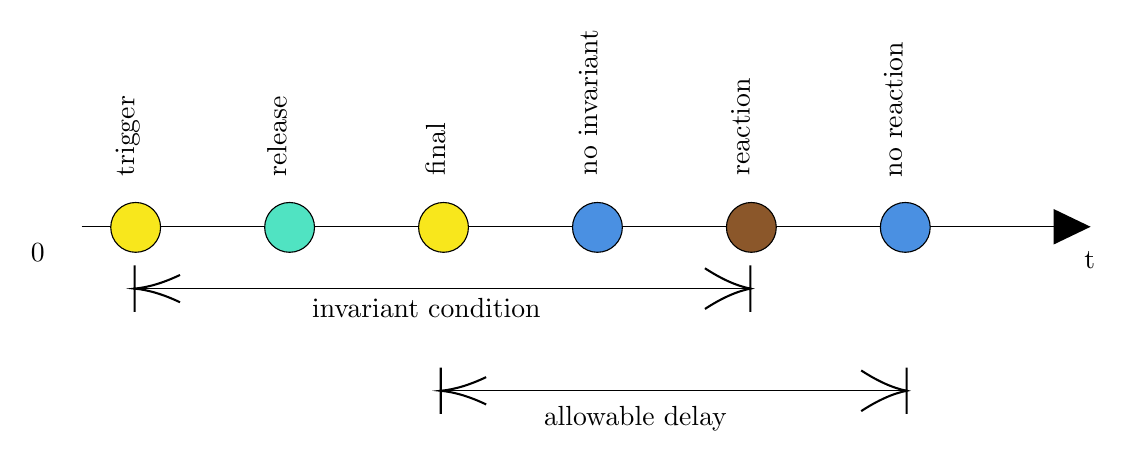
\begin{tikzpicture}[x=0.75pt,y=0.75pt,yscale=-2,xscale=2]
%uncomment if require: \path (0,300); %set diagram left start at 0, and has height of 300

%Straight Lines [id:da8140990256960691] 
\draw    (169.67,179.67) -- (409.72,179.67) ;
\draw [shift={(412.72,179.67)}, rotate = 180] [fill={rgb, 255:red, 0; green, 0; blue, 0 }  ][line width=0.08]  [draw opacity=0] (8.93,-4.29) -- (0,0) -- (8.93,4.29) -- cycle    ;
%Shape: Circle [id:dp6010009542999377] 
\draw  [fill={rgb, 255:red, 248; green, 231; blue, 28 }  ,fill opacity=1 ] (176.68,179.82) .. controls (176.68,176.5) and (179.37,173.82) .. (182.68,173.82) .. controls (186,173.82) and (188.68,176.5) .. (188.68,179.82) .. controls (188.68,183.13) and (186,185.82) .. (182.68,185.82) .. controls (179.37,185.82) and (176.68,183.13) .. (176.68,179.82) -- cycle ;
%Shape: Circle [id:dp34027802428728005] 
\draw  [fill={rgb, 255:red, 80; green, 227; blue, 194 }  ,fill opacity=1 ] (213.76,179.82) .. controls (213.76,176.5) and (216.45,173.82) .. (219.76,173.82) .. controls (223.08,173.82) and (225.76,176.5) .. (225.76,179.82) .. controls (225.76,183.13) and (223.08,185.82) .. (219.76,185.82) .. controls (216.45,185.82) and (213.76,183.13) .. (213.76,179.82) -- cycle ;
%Shape: Circle [id:dp11899817595493134] 
\draw  [fill={rgb, 255:red, 248; green, 231; blue, 28 }  ,fill opacity=1 ] (250.84,179.82) .. controls (250.84,176.5) and (253.53,173.82) .. (256.84,173.82) .. controls (260.16,173.82) and (262.84,176.5) .. (262.84,179.82) .. controls (262.84,183.13) and (260.16,185.82) .. (256.84,185.82) .. controls (253.53,185.82) and (250.84,183.13) .. (250.84,179.82) -- cycle ;
%Shape: Circle [id:dp012469973516187838] 
\draw  [fill={rgb, 255:red, 74; green, 144; blue, 226 }  ,fill opacity=1 ] (287.92,179.82) .. controls (287.92,176.5) and (290.61,173.82) .. (293.92,173.82) .. controls (297.24,173.82) and (299.92,176.5) .. (299.92,179.82) .. controls (299.92,183.13) and (297.24,185.82) .. (293.92,185.82) .. controls (290.61,185.82) and (287.92,183.13) .. (287.92,179.82) -- cycle ;
%Shape: Circle [id:dp07022441012642988] 
\draw  [fill={rgb, 255:red, 139; green, 87; blue, 42 }  ,fill opacity=1 ] (325,179.82) .. controls (325,176.5) and (327.69,173.82) .. (331,173.82) .. controls (334.32,173.82) and (337,176.5) .. (337,179.82) .. controls (337,183.13) and (334.32,185.82) .. (331,185.82) .. controls (327.69,185.82) and (325,183.13) .. (325,179.82) -- cycle ;
%Shape: Circle [id:dp9498629999029494] 
\draw  [fill={rgb, 255:red, 74; green, 144; blue, 226 }  ,fill opacity=1 ] (362.08,179.82) .. controls (362.08,176.5) and (364.77,173.82) .. (368.08,173.82) .. controls (371.4,173.82) and (374.08,176.5) .. (374.08,179.82) .. controls (374.08,183.13) and (371.4,185.82) .. (368.08,185.82) .. controls (364.77,185.82) and (362.08,183.13) .. (362.08,179.82) -- cycle ;
%Straight Lines [id:da5123896972610188] 
\draw    (182.43,194.57) -- (330.75,194.57) ;
\draw [shift={(330.75,194.57)}, rotate = 180] [color={rgb, 255:red, 0; green, 0; blue, 0 }  ][line width=0.75]    (0,5.59) -- (0,-5.59)(10.93,-4.9) .. controls (6.95,-2.3) and (3.31,-0.67) .. (0,0) .. controls (3.31,0.67) and (6.95,2.3) .. (10.93,4.9)   ;
\draw [shift={(182.43,194.57)}, rotate = 0] [color={rgb, 255:red, 0; green, 0; blue, 0 }  ][line width=0.75]    (0,5.59) -- (0,-5.59)(10.93,-3.29) .. controls (6.95,-1.4) and (3.31,-0.3) .. (0,0) .. controls (3.31,0.3) and (6.95,1.4) .. (10.93,3.29)   ;
%Straight Lines [id:da3462342407884763] 
\draw    (256.18,219.18) -- (368.39,219.18) ;
\draw [shift={(368.39,219.18)}, rotate = 180] [color={rgb, 255:red, 0; green, 0; blue, 0 }  ][line width=0.75]    (0,5.59) -- (0,-5.59)(10.93,-4.9) .. controls (6.95,-2.3) and (3.31,-0.67) .. (0,0) .. controls (3.31,0.67) and (6.95,2.3) .. (10.93,4.9)   ;
\draw [shift={(256.18,219.18)}, rotate = 0] [color={rgb, 255:red, 0; green, 0; blue, 0 }  ][line width=0.75]    (0,5.59) -- (0,-5.59)(10.93,-3.29) .. controls (6.95,-1.4) and (3.31,-0.3) .. (0,0) .. controls (3.31,0.3) and (6.95,1.4) .. (10.93,3.29)   ;

% Text Node
\draw (410.6,184.9) node [anchor=north west][inner sep=0.75pt]   [align=left] {t};
% Text Node
\draw (177.18,168.11) node [anchor=north west][inner sep=0.75pt]  [font=\normalsize,rotate=-270.31] [align=left] {trigger};
% Text Node
\draw (213.68,168.11) node [anchor=north west][inner sep=0.75pt]  [font=\normalsize,rotate=-270.31] [align=left] {release};
% Text Node
\draw (251.93,167.86) node [anchor=north west][inner sep=0.75pt]  [font=\normalsize,rotate=-270.31] [align=left] {final};
% Text Node
\draw (288.68,167.86) node [anchor=north west][inner sep=0.75pt]  [font=\normalsize,rotate=-270.31] [align=left] {no invariant};
% Text Node
\draw (325.43,167.86) node [anchor=north west][inner sep=0.75pt]  [font=\normalsize,rotate=-270.31] [align=left] {reaction};
% Text Node
\draw (362.18,168.36) node [anchor=north west][inner sep=0.75pt]  [font=\normalsize,rotate=-270.31] [align=left] {no reaction};
% Text Node
\draw (224.55,196.17) node [anchor=north west][inner sep=0.75pt]  [font=\normalsize] [align=center] {invariant condition};
% Text Node
\draw (280.39,222.27) node [anchor=north west][inner sep=0.75pt]  [font=\normalsize] [align=center] {allowable delay};
% Text Node
\draw (156.8,183.17) node [anchor=north west][inner sep=0.75pt]   [align=left] {0};


\end{tikzpicture}

    \caption{Диаграмма EDTL-требования} % Подпись к рисунку
    \label{fig:edtl_diagram} % Метка для ссылок в тексте (напр. рис. \ref{fig:edtl_diagram})
\end{figure}

\begin{definition}[Синтаксис термов EDTL]\label{def:edtl_terms}

    Множество корректных EDTL-термов определяется рекурсивно:
    \begin{itemize}
        \item любая константа или переменная типа $T$ по определению является термом типа $T$;
        \item если $u_1, \dots, u_n$~--- это термы типов $T_1, \dots, T_n$ соответственно, а $f$~--- функция с сигнатурой $T_1 \times \dots \times T_n \to T$, то результат применения функции $f(u_1, \dots, u_n)$ формирует новый терм целевого типа $T$;
        \item выражение $(u)$, где $u$~--- допустимый терм, также является термом исходного типа.
    \end{itemize}
    В качестве функций могут выступать стандартные арифметические операторы, операции отношения, а также базовые логические и побитовые операции.
\end{definition}

\begin{definition}[EDTL-формулы]\label{def:edtl_formulas}
    EDTL-формулы конструируются на основе логических термов с использованием стандартных булевых связок. 
    
    Пусть $\phi$ и $\psi$~--- корректные EDTL-формулы. Тогда правила построения формул задаются следующим образом:
    \begin{itemize}
        \item любой EDTL-терм типа \texttt{bool} выступает в роли атомарной EDTL-формулы;
        \item $\neg\phi$, $\phi \land \psi$ и $\phi \lor \psi$ также являются допустимыми формулами;
        \item $/\phi$~--- $\phi$ изменяет значение с истинного на ложное;
        \item $\backslash\phi$~--- $\phi$ изменяет значение с ложного на истинное);
        \item $\sim\phi$~--- значение $\phi$ сохраняется истинным;
        \item $\_\phi$~--- значение $\phi$ сохраняется ложным.
    \end{itemize}
\end{definition}


Для проведения анализа спецификаций паттерны EDTL имеют интерпретацию в линейной темпоральной логике (LTL). Требование $R$ считается выполненным для целевой системы, если на всех ее возможных начальных путях выполнения удовлетворяется следующая LTL-формула $\Phi_{R}$:
\begin{equation}\label{eq:edtl2ltl}
\begin{split}
    \Phi_R = \mathcal{G} \Big( &(\mathit{trigger} \land \neg \mathit{release}) \to \\
    \to \big( &(\mathit{invariant} \land \neg \mathit{final}) \ \mathcal{W} \ (\mathit{release} \lor {}\\
    {} \lor &(\mathit{final} \land ((\mathit{invariant} \land \neg \mathit{delay}) \ \mathcal{W} \ (\mathit{release} \lor {}\\
    {} \lor &(\mathit{invariant} \land \mathit{reaction}))))) \big) \Big)
\end{split}
\end{equation}

Где $\mathcal{G}$ (Globally), $\mathcal{U}$ (Until) и $\mathcal{W}$ (Weak Until)~--- стандартные операторы линейной темпоральной логики. Именно трансляция EDTL-паттернов в подобные громоздкие LTL-выражения делает актуальной задачу автоматизированной проверки результирующего множества формул на отсутствие логических конфликтов и избыточных ограничений.
\subsection{Существующие работы}\label{sec:related-work}

\todo{For the next deadline}

\subsection{Теорема Пифагора}\label{sec:pythagoras}



Основная формулировка содержит алгебраические действия --- в
прямоугольном треугольнике, длины катетов которого равны \(a\) и \(b\),
а длина гипотенузы --- \(c\), выполнено соотношение:

\[
a^2 + b^2 = c^2.
\]

Для того чтобы ссылаться на формулы, их можно нумеровать следующим
образом:

\begin{equation}\label{eq:pythagoras}{
a^2 + b^2 = c^2
}\end{equation}

Теперь можно сослаться на формулу~\eqref{eq:pythagoras} где угодно в
тексте.

\subsection{Пример листинга}\label{sec:lst-example}

Ниже в листинге~\ref{lst:python-fact} представлен пример вычисления
факториала на языке Python.

\begin{lstlisting}[language=Python, caption={Вычисление факториала числа n}, label=lst:python-fact]
def fact(n):
  if (n==1 or n==0):
    return 1
  else:
    return n * fact(n - 1)
\end{lstlisting}

\subsection{Пример рисунка}\label{sec:fig-example}

Далее на рис.~\ref{fig:png-svg-compare}~и~\ref{fig:tikz-example}
представлены примеры вставки изображений в работу.

\begin{figure}\centering%

\subfloat[]{\includegraphics[width=0.4\textwidth,height=\textheight]{images/sample/Markdown-mark.svg.png}\label{fig:markdown-mark-png}}
\subfloat[]{\includegraphics{images/sample/Markdown-mark.pdf}\label{fig:markdown-mark-svg}}

\caption{Пример рисунка в формате png \ref{fig:markdown-mark-png} и в
формате svg после конвертации в pdf
\ref{fig:markdown-mark-svg}}\label{fig:png-svg-compare}

\end{figure}

Всегда лучше выбирать рисунки в векторном формате (.svg, .pdf и.т.п),
либо рисовать прямо в \LaTeX\ с помощью Ti\emph{k}Z, как показано на
рис.~\ref{fig:tikz-example}.

\begin{tikzfigure}{fig:tikz-example}{Таблица виртуальных методов для класса C}
  {every node/.style={text=black}}

  \begin{scope}[blend group = soft light]
    \fill[red!30!white]   ( 90:1.2) circle (2);
    \fill[green!30!white] (210:1.2) circle (2);
    \fill[blue!30!white]  (330:1.2) circle (2);
  \end{scope}
  \node at ( 90:2)    {Typography};
  \node at ( 210:2)   {Design};
  \node at ( 330:2)   {Coding};
  \node [font=\Large] {\LaTeX};

\end{tikzfigure}

\clearpage
\pagebreak

\section{Постановка задачи}\label{sec:problem}
Поскольку любое EDTL-требование транслируется в формулу LTL \eqref{eq:edtl2ltl}, будем считать, что на входе мы имеем набор LTL-формул $\Phi$.

Целью данной работы является разработка программного решения, выполняющего автоматический анализ набора LTL-формул $\Phi$ на избыточность и противоречивость:
\begin{enumerate}
    \item Анализ на противоречивость. Для каждой формулы $\varphi \in \Phi$ необходимо найти:
    \begin{itemize}
        \item все минимальные невыполнимые подмножества (Minimal Unsatisfiable Subsets, MUS) $\Phi_1, \dots, \Phi_k \subset \Phi \setminus \{\varphi\}$ такие, что совместное выполнение $\varphi$ и всех элементов $\Phi_i$ невозможно (конъюнкция не имеет модели);
        \item все максимальные выполнимые подмножества (Maximal Satisfiable Subsets, MSS) $\Phi_1, \dots, \Phi_l \subset \Phi \setminus \{\varphi\}$ такие, что совместное выполнение $\varphi$ и всех элементов $\Phi_i$ допустимо (конъюнкция имеет модель).
    \end{itemize}

    \item Анализ на избыточность. Необходимо выявить все спецификации $\varphi \in \Phi$, наличие которых в исходном множестве не влияет на общее поведение системы, так как они логически выводятся из других требований. Формально требуется найти все такие $\varphi$, для которых в множестве $\Phi$ существует минимальное покрывающее подмножество $\Phi'$ ($\varphi \notin \Phi'$), удовлетворяющее условию:
    $$ \Phi' \models \varphi \land (\forall \varphi' \in \Phi' \colon \Phi' \setminus \{\varphi'\} \not\models \varphi). $$
\end{enumerate}

Для достижения поставленной цели необходимо решить следующие задачи:
\begin{enumerate}
    \item Изучить математический аппарат формализации требований: проанализировать синтаксис, семантику и выразительные возможности линейной темпоральной логики (LTL) и событийно-управляемой темпоральной логики (EDTL), а также способы трансляции EDTL-паттернов в LTL-представление.
    
    \item Исследовать методы локализации логических конфликтов: изучить теорию извлечения минимальных невыполнимых (MUS) и максимальных выполнимых (MSS) подмножеств.
    
    \item Проанализировать алгоритм MARCO (Mapping Regions of Constraints): разобрать логику навигации по пространству подмножеств (функции сжатия \texttt{Shrink} и расширения \texttt{Grow}), механизмы блокирующих клозов и абстракцию решателя (солвера).
    
    \item Изучить программные средства верификации: исследовать алгоритмы проверки выполнимости LTL-формул (в том числе теорию автоматов Бюхи) и освоить внутреннее устройство и программный интерфейс библиотеки Spot.
    
    \item Разработать метод и архитектуру решения: спроектировать интеграцию алгоритма MARCO с LTL-солвером Spot таким образом, чтобы абстрактный алгоритм перечисления MUS/MSS мог корректно обрабатывать спецификации темпоральной логики для выявления избыточности и противоречивости.
    
    \item Реализовать программный инструмент: написать исходный код приложения, реализующего разработанный метод автоматизированного контроля качества требований.
    
    \item Провести тестирование: верифицировать корректность работы созданного инструмента на тестовых наборах спецификаций и проанализировать полученные результаты.
\end{enumerate}
\section{РАЗРАБОТАННЫЙ ПОДХОД}\label{sec:solution}

\subsection{Определения}\label{sec:definitions}

\begin{definition}\label{def:even} Четным числом называется целое число, которое представимо
в виде произведения числа 2 и другого целого числа.
\end{definition}

\begin{definition}\label{def:odd} Нечетным числом называется целое
число, которое \textbf{не} представимо в виде произведения числа 2 и
другого целого числа.
\end{definition}

\subsection{Теоремы}\label{sec:theorems}

\begin{theorem}\label{thm:even} Сумма двух четных целых всегда четная.
\end{theorem}

\begin{proof} Пусть даны два целых числа $x, y \in \mathbb{Z}$. По определению\ \ref{def:even},
существуют такие целые числа $a, b \in \mathbb{Z}$, что $x$ и $y$ могут быть записаны следующим образом:
$$
\begin{aligned}
x &= 2a \\
y &= 2b
\end{aligned}
$$

Тогда их сумма также удовлетворяет определению\ \ref{def:even},
а значит является четным числом:
$$
x + y = 2a + 2b = 2(a + b).
$$
\end{proof}

\begin{corollary}\label{cor:even} Сумма $n$ четных целых всегда четная.
\end{corollary}

\subsection{Алгоритмы}\label{sec:algorithms}

Далее приведен алгорим~\ref{alg:gcd} для вычисления наибольшего общего
делителя.

\begin{algorithm}{alg:gcd} Поиск наибольшего общего делителя (НОД) двух
неотрицательных целых чисел \(a\) и \(b\), где \(a > b\).

\begin{enumerate}
\tightlist
\item
  Инициализировать переменные \(a\) и \(b\) аргументами;
\item
  Пока \(b \neq 0\):

  \begin{enumerate}
  \tightlist
  \item
    Вычислить остаток \(r\) от деления \(a\) на \(b\):
    \(r \gets a \mod b\);
  \item
    Обновить переменные \(a \gets b\), \(b \gets r\);
  \end{enumerate}
\item
  Вернуть значение \(a\) в качестве результата.
\end{enumerate}

\end{algorithm}

\clearpage
\pagebreak

\section{РЕЗУЛЬТАТЫ}\label{sec:results}

Тут приводится некоторое описание проведенных замеров, окружение, в
котором они проводились и представляются итоговые результаты\footnote{В
  тексте работы лучше приводить не только отрендеренные графики, но и
  таблицы с финальными данными, а также доверительные интервалы для
  каждой метрики.}.

\begin{longtable}[]{@{}lrrr@{}}
\caption{Замеры производительности бенчмарка
\passthrough{\lstinline!Bench!}}\tabularnewline
\toprule\noalign{}
Версия & Время (сек) & Кол-во запросов в сек. & Точность (\%) \\
\midrule\noalign{}
\endfirsthead
\toprule\noalign{}
Версия & Время (сек) & Кол-во запросов в сек. & Точность (\%) \\
\midrule\noalign{}
\endhead
\bottomrule\noalign{}
\endlastfoot
Base & 12.34 & 567 & 0.89 \\
Opt & 10.12 & 600 & 0.95 \\
Opt+ & \textbf{9.87} & \textbf{610} & \textbf{0.98} \\
Deopt & 15.67 & 520 & 0.75 \\
\end{longtable}

Также приводится анализ полученных результатов, в котором полезно
подчеркнуть не только замеры на которых произошли улучшения или
ухудшения, но и почему они там произошли, и как можно было бы этого
избежать.

\clearpage
\pagebreak

\section*{ЗАКЛЮЧЕНИЕ}\label{sec:conclusion}
\addcontentsline{toc}{section}{ЗАКЛЮЧЕНИЕ}

Основные результаты работы:

\begin{itemize}
\tightlist
\item
  Первый результат;
\item
  Второй результат;
\item
  Третий результат;
\item
  Последний результат.
\end{itemize}

Направление дальнейших работ:

\begin{itemize}
\tightlist
\item
  Улучшить алгоритм;
\item
  Провести анализ данных.
\end{itemize}

\clearpage
\pagebreak

\section*{СПИСОК ИСПОЛЬЗОВАННЫХ ИСТОЧНИКОВ}\label{sec:bib}
\addcontentsline{toc}{section}{СПИСОК ИСПОЛЬЗОВАННЫХ ИСТОЧНИКОВ}

\printbibliography[heading=none]

\renewcommand{\thesection}{П}
\setcounter{subsection}{0}
\setcounter{figure}{0}
\setcounter{lstlisting}{0}
\pagebreak

\section*{ПРИЛОЖЕНИЕ}\label{sec:appendix}
\addcontentsline{toc}{section}{ПРИЛОЖЕНИЕ}

\subsection{Первая глава приложения}\label{sec:appendix-1}

В приложение обычно выносятся длинные листинги и таблицы.

\end{document}
